\documentclass{ppgeesa}

\usepackage[hidelinks]{hyperref}
\usepackage{url}
\usepackage{breakurl}

\usepackage[detect-weight,detect-family]{siunitx}
\sisetup{output-decimal-marker = {,}}
\sisetup{exponent-product = {\cdot}}
\sisetup{group-digits = none}
\sisetup{round-mode = figures}
\sisetup{round-precision = 6}
\sisetup{round-pad = false}

\usepackage{amsmath}
\usepackage{amssymb}
\usepackage{mathtools}
\usepackage{resizegather}
\usepackage{icomma}
\mathtoolsset{showonlyrefs}
\newcommand{\Prod}{\,}

\usepackage{graphicx}
\usepackage{epstopdf}
\graphicspath{{../img/}}
\epstopdfsetup{outdir=./build/}

\usepackage[inline]{enumitem}

\usepackage{tabularx}
\usepackage{booktabs}

\hyphenation{ARX ARMAX OE BJ}

\begin{document}
\bstctlcite{IEEEBST:Brazilian}

\title{Identificação de Sistema por Erro de Predição com Modelos Racionais}
\author{Guilherme de Paoli Beal
  \\
  {\small Universidade Federal do Rio Grande do Sul
  \\
  Programa de Pós-Graduação em Engenharia Elétrica
  \\
  Aprendizado Supervisionado de Modelos Paramétricos}
  \thanks{G. Beal, guilherme.beal@ufrgs.br}
}
\maketitle
\thispagestyle{empty}\pagestyle{empty}

\begin{abstract}
  Este trabalho busca identificar um sistema por erro de predição, a partir de um conjunto de dados de entrada e saída, com a saída corrompida por ruído de medição.
  As classes de modelo ARX, ARMAX, Output Error e Box-Jenkins, com diferentes ordens, são avaliadas.
  As identificações são realizadas pelo pacote \texttt{pysid} em linguagem Python.
  Os resultados são comparados pelo erro quadrático médio de predição e pelo critério de informação de Akaike ajustado para dados com poucas amostras.
\end{abstract}

\begin{IEEEkeywords}
  Identificação por Erro de Predição, pysid, ARX, ARMAX, Output Error, Box-Jenkins
\end{IEEEkeywords}

\section{Introdução}

%% TODO desenvolver introdução
Este trabalho visa à aplicação de identificação de um sistema discreto, linear e invariante no tempo, através do método de erro de predição, ou \emph{Prediction Error Method} (PEM).
Uma batelada de dados de um sistema, supostamente desconhecido, é fornecida, em que a saída está contaminada por ruído de medição.
A identificação é realizada utilizando diferentes classes de modelo e ordens e os resultados são comparados.

As implementações são desenvolvidas em Python, versão 3.9.12.
A identificação por erro de predição utiliza o pacote \texttt{pysid} em versão de desenvolvimento 0.1.0.
O código deste projeto está publicado em \href{https://github.com/GuiBeal/system-identification}{\texttt{github.com/GuiBeal/system-identification}}.

\section{Identificação por Erro de Predição}

Considere um sistema discreto, linear, invariante no tempo, com uma única entrada e uma única saída.
A resposta deste sistema é dada por
\begin{equation}\label{eq:system}
  y(t) = G_0(q) \Prod u(t) + \nu(t)
  ,\; t \in \mathbb{N}
  ,
\end{equation}
em que
$y(t)$ é o sinal de saída,
$G_0(q)$ é a função de transferência do sistema,
$u(t)$ é o sinal de entrada,
$\nu(t)$ é um ruído de medição desconhecido, %% TODO verificar nomenclatura
$q$ é o operador de avanço --- de modo que $q \Prod x(t) = x(t+1)$ --- e
$t \in \mathbb{N}$ é a variável de tempo discreto.
O ruído de medição é gerado a partir de ruído branco filtrado, como
\begin{equation}
  \nu(t) = H_0(q) \Prod e(t)
  ,
\end{equation}
em que
$H_0(q)$ é a função de transferência do filtro e
$e(t)$ é ruído branco.

\subsection{Modelos Racionais}

O modelo busca representar o sistema real $G_0(q)$ expresso em \eqref{eq:system}.
Em particular, na identificação por erro de predição, o modelo procurar caracterizar também o ruído $\nu(t)$ através da identificação de $H_0(q)$.

Quatro diferentes classes de modelo racionais são exploradas neste trabalho:
\begin{itemize}
  \item Autorregressivo com Entrada Externa, ou \emph{Autoregressive with Extra Input} (ARX);
  \item Autorregressivo com Média Móvel e Entrada Externa, ou \emph{Autoregressive Moving Average with Extra Input} (ARMAX);
  \item Erro na Saída, ou \emph{Output Error} (OE); e
  \item Box-Jenkins (BJ).
\end{itemize}
Essas classes são casos particulares de um modelo mais genérico, definido por
\begin{equation}\label{eq:model}
  A(q) \Prod y(t) = \dfrac{B(q)}{F(q)} \Prod u(t) + \dfrac{C(q)}{D(q)} \Prod e(t)
  .
\end{equation}
Os polinômios têm os formatos
\begin{align}
  A(q) &= 1 + a_1 \Prod q^{-1} + \dotsb + a_{n_a} \Prod q^{-n_a}
  ,
  \\
  B(q) &= q^{-n_k} \Prod \left(b_0 + b_1 \Prod q^{-1} + \dotsb + b_{n_b} \Prod q^{-n_b}\right)
  ,
  \\
  C(q) &= 1 + c_1 \Prod q^{-1} + \dotsb + c_{n_c} \Prod q^{-n_c}
  ,
  \\
  D(q) &= 1 + d_1 \Prod q^{-1} + \dotsb + d_{n_d} \Prod q^{-n_d}
  , \text{ e}
  \\
  F(q) &= 1 + f_1 \Prod q^{-1} + \dotsb + f_{n_f} \Prod q^{-n_f}
  ,
\end{align}
em que $n_a$, $n_b$, $n_c$, $n_d$ e $n_f$ são suas ordens e $n_k$ é o número de atrasos da entrada para a saída.
Definindo as funções de transferência
\begin{align}
  G(q) &= \dfrac{B(q)}{A(q) \Prod F(q)}
  , \text{ e}
  \\
  H(q) &= \dfrac{C(q)}{A(q) \Prod D(q)}
  ,
\end{align}
então \eqref{eq:model} pode ser reescrita como
\begin{equation}\label{eq:model-tf}
  y(t) = G(q) \Prod u(t) + H(q) \Prod e(t)
  .
\end{equation}
Note que $G(q)$ visa a caracterizar o sistema real $G_0(q)$.
Por sua vez, o ruído de medição $\nu(t)$ é representado como ruído branco $e(t)$ filtrado por $H(q)$.

Pelas definições dos polinômios,
\begin{equation}\label{eq:H-inf}
  H(\infty) = 1
  .
\end{equation}
Outrossim, se o modelo representa um sistema amostrado, então $G(q)$ deve ser estritamente própria --- isto é, o grau de seu denominador é maior que o de seu numerador --- o que é garantido com $n_k \geq 1$.

Ressalta-se que este modelo genérico pode apresentar definições e notações diferentes, como em \cite{book:Ljung1999, book:Aguirre2007, misc:matlab-polynomial-models}.
A definição aqui apresentada corresponde ao formato dos polinômios retornados pelas funções do pacote \texttt{pysid}.

\subsection{Predição}

A predição é realizada aplicando
\begin{equation}\label{eq:prediction}
  \hat{y}(t) = L_u(q) \Prod u(t) + L_y(q) \Prod y(t)
\end{equation}
com
\begin{align}
  L_u(q) &= \dfrac{G(q)}{H(q)}
  , \text{ e}
  \\
  L_y(q) &= 1 - \dfrac{1}{H(q)}
  .
\end{align}
Embora isso não seja diretamente evidenciado por \eqref{eq:prediction}, o fato de $G(q)$ ser estritamente própria juntamente com \eqref{eq:H-inf} garante que a predição $\hat{y}(t)$ no instante $t = t_0$ depende somente de valores de $u(t)$ e $y(t)$ em instantes $t < t_0$ --- isto é, a predição é realizado a partir de valores anteriores dos sinais de entrada e saída medidos.

O erro de predição é definido como
\begin{equation}
  \varepsilon(t)
  = y(t) - \hat{y}(t)
  = \dfrac{y(t) - G(q) \Prod u(t)}{H(q)}
  .
\end{equation}
Assim, o erro quadrático médio de predição é definido por
\begin{equation}\label{eq:mse}
  J = \dfrac{1}{N} \Prod \sum_{t=1}^{N}{\left(\varepsilon(t)\right)^2}
  ,
\end{equation}
em que $N$ é o número de amostras preditas.

\subsection{Identificação}
A identificação por erro de predição visa, a partir de um conjunto de dados de entrada $u(t)$ e de saída $y(t)$ medidos do processo, a identificar os parâmetros dos polinômios do modelo de forma a minimizar o custo expresso em \eqref{eq:mse}.
O algoritmo aplicado neste processo depende da classe do modelo e está fora do escopo deste trabalho.
Estes são implementados pelo pacote \texttt{pysid}.

\subsection{Classes de Modelos}
As quatro classes de modelo são obtidas fixando determinadas ordens no modelo genérico.

\subsubsection{ARX}
Neste modelo, há liberdade nas escolhas de $n_a$, $n_b$ e $n_k$, enquanto $n_c = n_d = n_f = 0$.
Assim, as funções de transferência tornam-se
\begin{align}
  G(q) &= \dfrac{B(q)}{A(q)}
  , \text{ e}
  \\
  H(q) &= \dfrac{1}{A(q)}
  .
\end{align}
Esta classe tem a vantagem de fazer com que \eqref{eq:mse} seja quadrática nos parâmetros, os quais podem, portanto, ser calculados por mínimos quadrados.

\subsubsection{ARMAX}
Este modelo requer a arbitração das ordens $n_a$, $n_b$, $n_c$ e $n_k$, com $n_d = n_f = 0$.
Portanto, as funções de transferência são
\begin{align}
  G(q) &= \dfrac{B(q)}{A(q)}
  , \text{ e}
  \\
  H(q) &= \dfrac{C(q)}{A(q)}
  .
\end{align}

\subsubsection{\emph{Output Error}}
Para este modelo são escolhidas as ordens $n_b$, $n_f$ e $n_k$, fixando $n_a = n_c = n_d = 0$.
Nesse casso, tem-se
\begin{align}
  G(q) &= \dfrac{B(q)}{F(q)}
  , \text{ e}
  \\
  H(q) &= 1
  .
\end{align}
Note que este modelo considera que o ruído de medição é ruído branco. % TODO nomenclatura

\subsubsection{Box-Jenkins}
Finalmente, neste modelo arbitra-se $n_b$, $n_c$, $n_d$, $n_f$ e $n_k$, com $n_a = 0$.
Com isso, obtém-se
\begin{align}
  G(q) &= \dfrac{B(q)}{F(q)}
  , \text{ e}
  \\
  H(q) &= \dfrac{C(q)}{D(q)}
  .
\end{align}

\section{Critério de Informação de Akaike}

Para avaliar a qualidade dos modelos identificados será utilizado o critério de informação de Akaike, ou \emph{Akaike Information Criterion} (AIC).
Este critério pondera a qualidade de predição junto à ordem do modelo, penalizando critérios de maior ordem.
Considerando o erro de predição, o critério é definido por
\begin{equation}
  \text{AIC} = N \Prod \log\left(J\right) + 2 \Prod k
  ,
\end{equation}
em que $N$ é o número de amostras preditas, $k$ é o número de parâmetros do modelo e $J$ é o erro médio quadrático de predição definido em \eqref{eq:mse} \cite{book:Soderstrom1989}.

Para conjuntos com poucas amostras, pode-se utilizar um critério adaptado, definido por
\begin{equation}\label{eq:akaike-small}
  \text{AICc} = \text{AIC} + \dfrac{2 \Prod k \Prod \left(k + 1\right)}{N - k - 1}
  .
\end{equation}
Note que $N \to \infty \implies \text{AICc} \to \text{AIC}$ --- isto é, o critério adaptado se aproximado do critério original à medida que cresce o número de amostras considerado.

\section{Dados}

Os dados são apresentados na Figura \ref{fig:data}, em que o sinal $u(t)$ é multiplicado por um fator de $10$ para melhor visualização.
Ambos os sinais $u(t)$ e $y(t)$ contêm 200 amostras.
Note que a entrada $u(t)$ é similar a uma onda quadrada.
\begin{figure}[!htbp]
  \centering
  \includegraphics[width=\linewidth]{data_folded}
  \caption{Dados de entrada e saída.}
  \label{fig:data}
\end{figure}

Na Figura \ref{fig:data}, a linha tracejada vertical divide os dados em dois conjuntos.
Para a identificação dos modelos, utilizam-se os dados à esquerda desta linha, correspondentes às primeiras 160 amostras.
As 40 amostras restantes são aplicadas na validação dos modelos identificados.

A Figura \ref{fig:data_fourier} mostra o espectro de amplitude dos dados --- isto é, a magnitude da transformada de Fourier dos sinais --- em escala logarítmica.
Note como ambos os sinais possuem um conteúdo elevado em baixas frequências, seguidos de picos pontuais que decrescem com o aumento da frequência.
\begin{figure}[!htbp]
  \centering
  \includegraphics[width=\linewidth]{data_fourier_log}
  \caption{Espectro de amplitude dos dados de entrada e saída.}
  \label{fig:data_fourier}
\end{figure}

\section{Resultados}

Diversas identificações são realizadas, variando as ordens dos polinômios e o atraso entre as quatro classes de modelos.
A Tabela \ref{tab:orders} sintetiza os intervalos de variação desses valores para cada modelo.
% As ordens $n_a$, $n_d$ e $n_f$ variam a partir de 1.
% Note que, no modelo ARMAX, $n_c = 0$ equivaleria ao modelo ARX; portanto, essa ordem nesse modelo varia a partir de 1.
A fim de considerar sistemas amostrados, todos os sistemas tem atraso de pelo menos um amostra --- isto é, $n_k \geq 1$.

\begin{table}[!htbp]
  \centering
  \caption{Intervalo de variação das ordens dos polinômios}
  \label{tab:orders}
  \newcolumntype{C}{>{\centering\arraybackslash}X}
\setlength{\extrarowheight}{1pt}
\begin{tabularx}{\linewidth}{@{} c *{6}{C} c @{}}
  \toprule
  Classe & $n_a$    & $n_b$    & $n_c$    & $n_d$    & $n_f$    & $n_k$    & Total \\
  \midrule
  ARX    & $[1, 4]$ & $[0, 4]$ & --       & --       & --       & $[1, 4]$ & 80    \\
  ARMAX  & $[1, 4]$ & $[0, 4]$ & $[1, 4]$ & --       & --       & $[1, 4]$ & 320   \\
  OE     & --       & $[0, 4]$ & --       & --       & $[1, 4]$ & $[1, 4]$ & 80    \\
  BJ     & --       & $[0, 4]$ & $[0, 4]$ & $[1, 4]$ & $[1, 4]$ & $[1, 4]$ & 1600  \\
  \midrule
  Total  &          &          &          &          &          &          & 2080  \\
  \bottomrule
\end{tabularx}
\end{table}

Destaca-se que dentre as 1600 identificações realizadas com a classe BJ 960 apresentaram algum problema de implementação interno ao pacote \texttt{pysid}.
Nesses casos, os modelos foram descartados.
Assim, o total de modelos efetivamente identificados é de 1120.

Para cada identificação são calculados o erro quadrático médio, conforme \eqref{eq:mse}, e o critério de informação de Akaike para pequenos conjuntos de dados, conforme \eqref{eq:akaike-small}.
Ambos são realizados tanto para o conjunto de dados de identificação --- denotado pelo subíndice $i$ --- como para o conjunto de validação --- denotado pelo subíndice $v$.

Para cada uma das quatro classes, a Tabela \ref{tab:results-class} apresenta os seis melhores modelos resultantes, com base no critério de informação de Akaike com os dados de validação --- isto é, $\text{AICc}_v$.
% Os demais custos também constam na tabela.
Os modelos são unicamente identificados por um índice, exibidos na primeira coluna.

\begin{table*}
  \caption{Melhores resultados por classe com base no critério $\text{AICc}_v$}
  \label{tab:results-class}
  \newcolumntype{C}{>{\centering\arraybackslash}X}
\setlength{\extrarowheight}{1pt}
\begin{tabularx}{\textwidth}{@{} c c *{6}{C} c c c c @{}}
  \toprule
  \#   & Classe & $n_a$   & $n_b$   & $n_c$   & $n_d$   & $n_f$   & $n_k$   & $\text{AICc}_v$ & $\text{AICc}_i$ & $J_v$         & $J_i$        \\
  \midrule
  24   & ARX    & \num{2} & \num{1} & --      & --      & --      & \num{1} & \num{79.463 }   & \num{288.142}   & \num{5.801  } & \num{5.750 } \\
  44   & ARX    & \num{3} & \num{1} & --      & --      & --      & \num{1} & \num{80.358 }   & \num{289.971}   & \num{5.556  } & \num{5.740 } \\
  28   & ARX    & \num{2} & \num{2} & --      & --      & --      & \num{1} & \num{80.596 }   & \num{276.503}   & \num{5.589  } & \num{5.276 } \\
  20   & ARX    & \num{2} & \num{0} & --      & --      & --      & \num{1} & \num{80.820 }   & \num{290.423}   & \num{6.384  } & \num{5.910 } \\
  40   & ARX    & \num{3} & \num{0} & --      & --      & --      & \num{1} & \num{81.303 }   & \num{291.572}   & \num{6.074  } & \num{5.875 } \\
  32   & ARX    & \num{2} & \num{3} & --      & --      & --      & \num{1} & \num{82.077 }   & \num{278.289}   & \num{5.410  } & \num{5.264 } \\
  \midrule
  160  & ARMAX  & \num{2} & \num{0} & \num{1} & --      & --      & \num{1} & \num{82.406 }   & \num{292.387}   & \num{6.244  } & \num{5.905 } \\
  240  & ARMAX  & \num{3} & \num{0} & \num{1} & --      & --      & \num{1} & \num{82.440 }   & \num{291.698}   & \num{5.853  } & \num{5.802 } \\
  192  & ARMAX  & \num{2} & \num{2} & \num{1} & --      & --      & \num{1} & \num{83.302 }   & \num{278.685}   & \num{5.579  } & \num{5.277 } \\
  144  & ARMAX  & \num{1} & \num{4} & \num{1} & --      & --      & \num{1} & \num{83.435 }   & \num{299.330}   & \num{5.199  } & \num{5.922 } \\
  112  & ARMAX  & \num{1} & \num{2} & \num{1} & --      & --      & \num{1} & \num{83.574 }   & \num{294.450}   & \num{6.021  } & \num{5.902 } \\
  336  & ARMAX  & \num{4} & \num{1} & \num{1} & --      & --      & \num{1} & \num{84.031 }   & \num{282.669}   & \num{5.277  } & \num{5.337 } \\
  \midrule
  465  & OE     & --      & \num{4} & --      & --      & \num{1} & \num{2} & \num{203.538}   & \num{635.576}   & \num{112.710} & \num{49.103} \\
  469  & OE     & --      & \num{4} & --      & --      & \num{2} & \num{2} & \num{205.126}   & \num{637.238}   & \num{108.924} & \num{48.942} \\
  466  & OE     & --      & \num{4} & --      & --      & \num{1} & \num{3} & \num{208.209}   & \num{688.227}   & \num{126.671} & \num{68.237} \\
  468  & OE     & --      & \num{4} & --      & --      & \num{2} & \num{1} & \num{210.717}   & \num{620.915}   & \num{125.264} & \num{44.195} \\
  470  & OE     & --      & \num{4} & --      & --      & \num{2} & \num{3} & \num{211.195}   & \num{690.408}   & \num{126.771} & \num{68.234} \\
  464  & OE     & --      & \num{4} & --      & --      & \num{1} & \num{1} & \num{211.208}   & \num{622.115}   & \num{136.532} & \num{45.141} \\
  \midrule
  1136 & BJ     & --      & \num{2} & \num{0} & \num{2} & \num{1} & \num{1} & \num{82.909 }   & \num{276.778}   & \num{5.524  } & \num{5.214 } \\
  816  & BJ     & --      & \num{1} & \num{0} & \num{2} & \num{1} & \num{1} & \num{83.040 }   & \num{273.646}   & \num{5.941  } & \num{5.183 } \\
  832  & BJ     & --      & \num{1} & \num{0} & \num{3} & \num{1} & \num{1} & \num{84.041 }   & \num{276.120}   & \num{5.683  } & \num{5.193 } \\
  1456 & BJ     & --      & \num{3} & \num{0} & \num{2} & \num{1} & \num{1} & \num{84.939 }   & \num{277.505}   & \num{5.398  } & \num{5.167 } \\
  1140 & BJ     & --      & \num{2} & \num{0} & \num{2} & \num{2} & \num{1} & \num{85.844 }   & \num{278.965}   & \num{5.521  } & \num{5.214 } \\
  848  & BJ     & --      & \num{1} & \num{0} & \num{4} & \num{1} & \num{1} & \num{86.957 }   & \num{274.874}   & \num{5.677  } & \num{5.083 } \\
  \bottomrule
\end{tabularx}
\end{table*}

Comparando a ordem de grandeza de cada critério de qualidade na Tabela \ref{tab:results-class}, nota-se que os modelos ARX, ARMAX e BJ apresentam um desempenho consideravelmente melhor que os modelos OE;
isto é um indicativo de que o ruído de medição não é branco, conforme supõe esse último modelo.
Além disso, para os modelos ARX, ARMAX e BJ, todos as identificações presentes na Tabela \ref{tab:results-class} têm $n_k = 1$ --- isto é, um atraso da entrada para a saída de apenas uma amostra.
Destaca-se, ainda, que entre os modelos ARMAX e BJ presentes na Tabela \ref{tab:results-class} todas as identificações têm $n_c$ partindo de seu valor mínimo --- 1 para ARMAX e 0 para BJ ---, levando à interpretação de que o numerador de $H(q)$ tem ordem pequena.

A Tabela \ref{tab:results} mostra as 20 melhores identificações, novamente classificadas pelo critério de informação de Akaike adaptado com os dados de validação --- $\text{AICc}_v$.
Note a prevalência de modelos ARX, bem como das características discutidas no parágrafo anterior.

\begin{table*}
  \caption{Melhores resultados gerais com base no critério $\text{AICc}_v$}
  \label{tab:results}
  \newcolumntype{C}{>{\centering\arraybackslash}X}
\setlength{\extrarowheight}{1pt}
\begin{tabularx}{\textwidth}{@{} c c *{6}{C} c c c c @{}}
  \toprule
  \#   & Classe & $n_a$   & $n_b$   & $n_c$   & $n_d$   & $n_f$   & $n_k$   & $\text{AICc}_v$ & $\text{AICc}_i$ & $J_v$  & $J_i$       \\
  \midrule
  24   & ARX    & \num{2} & \num{1} &  --     &  --       &  --   & \num{1} & \num{79.463} & \num{288.142} & \num{5.801} & \num{5.750} \\
  44   & ARX    & \num{3} & \num{1} &  --     &  --       &  --   & \num{1} & \num{80.358} & \num{289.971} & \num{5.556} & \num{5.740} \\
  28   & ARX    & \num{2} & \num{2} &  --     &  --       &  --   & \num{1} & \num{80.596} & \num{276.503} & \num{5.589} & \num{5.276} \\
  20   & ARX    & \num{2} & \num{0} &  --     &  --       &  --   & \num{1} & \num{80.820} & \num{290.423} & \num{6.384} & \num{5.910} \\
  40   & ARX    & \num{3} & \num{0} &  --     &  --       &  --   & \num{1} & \num{81.303} & \num{291.572} & \num{6.074} & \num{5.875} \\
  32   & ARX    & \num{2} & \num{3} &  --     &  --       &  --   & \num{1} & \num{82.077} & \num{278.289} & \num{5.410} & \num{5.264} \\
  64   & ARX    & \num{4} & \num{1} &  --     &  --       &  --   & \num{1} & \num{82.145} & \num{288.495} & \num{5.419} & \num{5.611} \\
  160  & ARMAX  & \num{2} & \num{0} & \num{1} &  --       &  --   & \num{1} & \num{82.406} & \num{292.387} & \num{6.244} & \num{5.905} \\
  240  & ARMAX  & \num{3} & \num{0} & \num{1} &  --       &  --   & \num{1} & \num{82.440} & \num{291.698} & \num{5.853} & \num{5.802} \\
  1136 & BJ     &  --     & \num{2} & \num{0} & \num{2} & \num{1} & \num{1} & \num{82.909} & \num{276.778} & \num{5.524} & \num{5.214} \\
  816  & BJ     &  --     & \num{1} & \num{0} & \num{2} & \num{1} & \num{1} & \num{83.040} & \num{273.646} & \num{5.941} & \num{5.183} \\
  36   & ARX    & \num{2} & \num{4} &  --     &  --       &  --   & \num{1} & \num{83.283} & \num{281.484} & \num{5.179} & \num{5.297} \\
  192  & ARMAX  & \num{2} & \num{2} & \num{1} &  --       &  --   & \num{1} & \num{83.302} & \num{278.685} & \num{5.579} & \num{5.277} \\
  60   & ARX    & \num{4} & \num{0} &  --     &  --       &  --   & \num{1} & \num{83.403} & \num{291.217} & \num{5.995} & \num{5.784} \\
  144  & ARMAX  & \num{1} & \num{4} & \num{1} &  --       &  --   & \num{1} & \num{83.435} & \num{299.330} & \num{5.199} & \num{5.922} \\
  112  & ARMAX  & \num{1} & \num{2} & \num{1} &  --       &  --   & \num{1} & \num{83.574} & \num{294.450} & \num{6.021} & \num{5.902} \\
  48   & ARX    & \num{3} & \num{2} &  --     &  --       &  --   & \num{1} & \num{83.698} & \num{278.625} & \num{5.634} & \num{5.275} \\
  336  & ARMAX  & \num{4} & \num{1} & \num{1} &  --       &  --   & \num{1} & \num{84.031} & \num{282.669} & \num{5.277} & \num{5.337} \\
  832  & BJ     &  --     & \num{1} & \num{0} & \num{3} & \num{1} & \num{1} & \num{84.041} & \num{276.120} & \num{5.683} & \num{5.193} \\
  52   & ARX    & \num{3} & \num{3} &  --     &  --       &  --   & \num{1} & \num{84.774} & \num{280.442} & \num{5.376} & \num{5.263} \\
  \bottomrule
\end{tabularx}
\end{table*}

A partir das identificações, são obtidas as funções de transferência do sistema $G(q)$ e do ruído $H(q)$.
A fim de compará-las visualmente, as Figuras \ref{fig:bode-system} e \ref{fig:bode-noise} apresentam suas respostas em frequência, considerando as identificações na Tabela \ref{tab:results}.

\begin{figure}[!htbp]
  \centering
  \includegraphics[width=\linewidth]{bode_G_AICCv}
  \caption{Respostas em frequência de $G(q)$ a partir das identificações na Tabela \ref{tab:results}.}
  \label{fig:bode-system}
\end{figure}

\begin{figure}[!htbp]
  \centering
  \includegraphics[width=\linewidth]{bode_H_AICCv}
  \caption{Respostas em frequência de $H(q)$ a partir das identificações na Tabela \ref{tab:results}.}
  \label{fig:bode-noise}
\end{figure}

Note, através da Figura \ref{fig:bode-system}, que, entre todas as identificações, o comportamento do sistema $G(q)$ é semelhante nas baixas frequências mas discordante nas altas frequências.
Isso está em consonância com o fato de que os dados trazem mais informações nas baixas frequências, conforme visto na Figura \ref{fig:data_fourier}.
Por outro lado, a Figura \ref{fig:bode-noise} mostra que o sistema $H(q)$ é mais diverso entre as diferentes identificações.
% A identificação do ruído não é tão boa quanto a identificação do sistema.

As predições das identificações presentes na Tabela \ref{tab:results} são exibidas na Figura \ref{fig:prediction}.
Os respectivos erros de predição --- também denominados resíduos --- são mostrados na Figura \ref{fig:residue}.
Observe que, de forma geral, as predições das várias identificações são próximas entre si.

Finalmente, a Figura \ref{fig:residue-autocorrelation} exibe a autocorrelação dos resíduos.
Caso um modelo fosse capaz de explicar plenamente a dinâmica do sistema, então os resíduos decorreriam apenas da aleatoriedade do ruído de medição e seriam semelhantes a ruído branco --- o qual é descorrelacionado de si mesmo exceto para atraso nulo.
A autocorrelação dos resíduos, porém, mostra um valor elevado para atraso nulo --- conforme esperado --- e valores diversos nos demais atrasos, mostrando que o resíduo não se aproxima de ruído branco.
\begin{figure}[!htbp]
  \centering
  \includegraphics[width=\linewidth]{prediction_AICCv}
  \caption{Predições a partir das identificações na Tabela \ref{tab:results}.}
  \label{fig:prediction}
\end{figure}

\begin{figure}[!htbp]
  \centering
  \includegraphics[width=\linewidth]{residue_AICCv}
  \caption{Resíduos de predição a partir das identificações na Tabela \ref{tab:results}.}
  \label{fig:residue}
\end{figure}

\begin{figure}[!htbp]
  \centering
  \includegraphics[width=\linewidth]{residue_autocorrelation_AICCv}
  \caption{Autocorrelação dos resíduos de predição a partir das identificações na Tabela \ref{tab:results}.}
  \label{fig:residue-autocorrelation}
\end{figure}

\subsection{Escolha de Modelos Adequados}
Através das observações anteriores, procura-se escolher classes e ordens de modelo razoáveis para representar o sistema efetivo, ainda desconhecido.
Os modelos OE são logo descartados devido ao seu desempenho inferior.
Ademais, o atraso é arbitrado como $n_k = 1$ pois esse valor prevalece nos modelos bem-classificados.

Conforme já citado, o numerador de $H(q)$ parece ser de ordem pequena.
Em particular, com a prevalência de modelos BJ com $n_c = 0$ --- o que equivale a $C(q) = 1$, sem parâmetros --- e de modelos ARX, descarta-se também a classe ARMAX.
Restam, portanto, modelos ARX e modelos BJ com $n_c = 0$.
A diferença entre esses dois casos é que o primeiro requer que os denominadores de $G(q)$ e $H(q)$ sejam iguais, enquanto o segundo permite que sejam independentes.

Finalmente, por apresentar melhores classificações gerais com estrutura mais simples, sugere-se a utilização do modelo ARX.
Pelos resultados, sugere-se uma ordem $n_a$ entre 2 e 3.
A ordem $n_b$ pode ser arbitrada entre 0 e 3.
Ressalta-se que a escolha de ordens mais elevadas permite contemplar uma quantidade maior de modelos na classe, ao custo de exigir a identificação de mais parâmetros.
Conforme já mencionado, o atraso sugerido é $n_k = 1$.

\subsection{Desempenho do Menor Modelo de Ordem Completa}
As funções de transferência que efetivamente geraram os dados são agora reveladas como
\begin{align}
  G_0(q) &= \dfrac{                   \num{2} \Prod q^2 + \num{2} \Prod q      - \num{1.5}                    }{q^3 - \num{1.4} \Prod q^2    + \num{0.48} \Prod q     }
  \\
         &= \dfrac{q^{-1} \Prod \left(\num{2}           + \num{2} \Prod q^{-1} - \num{1.5} \Prod q^{-2}\right)}{1   - \num{1.4} \Prod q^{-1} + \num{0.48} \Prod q^{-2}}
  , \text{ e}
  \\
  H_0(q) &= \dfrac{q^3}{q^3 - \num{1.4} \Prod q^2    + \num{0.48} \Prod q     }
  \\
         &= \dfrac{1  }{1   - \num{1.4} \Prod q^{-1} + \num{0.48} \Prod q^{-2}}
  .
\end{align}
Observe que os denominadores de $G_0(q)$ e $H_0(q)$ são idênticos.
Além disso, no formato de potências negativas, o numerador de $H_0(q)$ é unitário.
Assim, a classe de modelo ARX com $n_a = 2$, $n_b = 2$ e $n_k = 1$ é a menor classe que contém o sistema efetivo.

Note, através das Tabelas \ref{tab:results-class} e \ref{tab:results}, que essa classe corresponde à identificação de índice 28.
Além disso, é a terceira melhor classificada tanto entre os modelos ARX como no geral.
Seus polinômios são
\begin{align}
  A_{28}(q) &= 1   - \num{1.40683412} \Prod q^{-1} + \num{0.48261202} \Prod q^{-2}
  , \text{ e}
  \\
  B_{28}(q) &= q^{-1} \Prod \left(\num{2.16246556} + \num{1.61084338} \Prod q^{-1} - \num{1.6016382} \Prod q^{-2}\right)
  ,
\end{align}
os quais resultam nas funções de transferência
\begin{align}
  G_{28}(q) &= \dfrac{                   \num{2.16246556} \Prod q^2 + \num{1.61084338} \Prod q      - \num{1.6016382}                    }{q^3 - \num{1.40683412} \Prod q^2    + \num{0.48261202} \Prod q     }
  \\
            &= \dfrac{q^{-1} \Prod \left(\num{2.16246556}           + \num{1.61084338} \Prod q^{-1} - \num{1.6016382} \Prod q^{-2}\right)}{1   - \num{1.40683412} \Prod q^{-1} + \num{0.48261202} \Prod q^{-2}}
  , \text{ e}
  \\
  H_{28}(q) &= \dfrac{q^3}{q^3 - \num{1.40683412} \Prod q^2    + \num{0.48261202} \Prod q     }
  \\
            &= \dfrac{1  }{1   - \num{1.40683412} \Prod q^{-1} + \num{0.48261202} \Prod q^{-2}}
  .
\end{align}

A Figura \ref{fig:prediction-complete} mostra a previsão da saída a partir desta identificação, em comparação aos dados de validação.
Conforme consta nas Tabelas \ref{tab:results-class} e \ref{tab:results}, o erro quadrático médio associado é $\num{5.589}$.
\begin{figure}[!htbp]
  \centering
  \includegraphics[width=\linewidth]{y_p_28}
  \caption{Previsão obtida com o menor modelo de ordem completa.}
  \label{fig:prediction-complete}
\end{figure}

A comparação com os sistemas efetivos é realizada pelas respostas em frequência das funções de transferência, as quais são exibidas nas Figuras \ref{fig:bode-system-complete} e \ref{fig:bode-noise-complete}.
Observe que a função $G_{28}(q)$ apresenta um ganho estático visivelmente abaixo de $G_0(q)$.
\begin{figure}[!htbp]
  \centering
  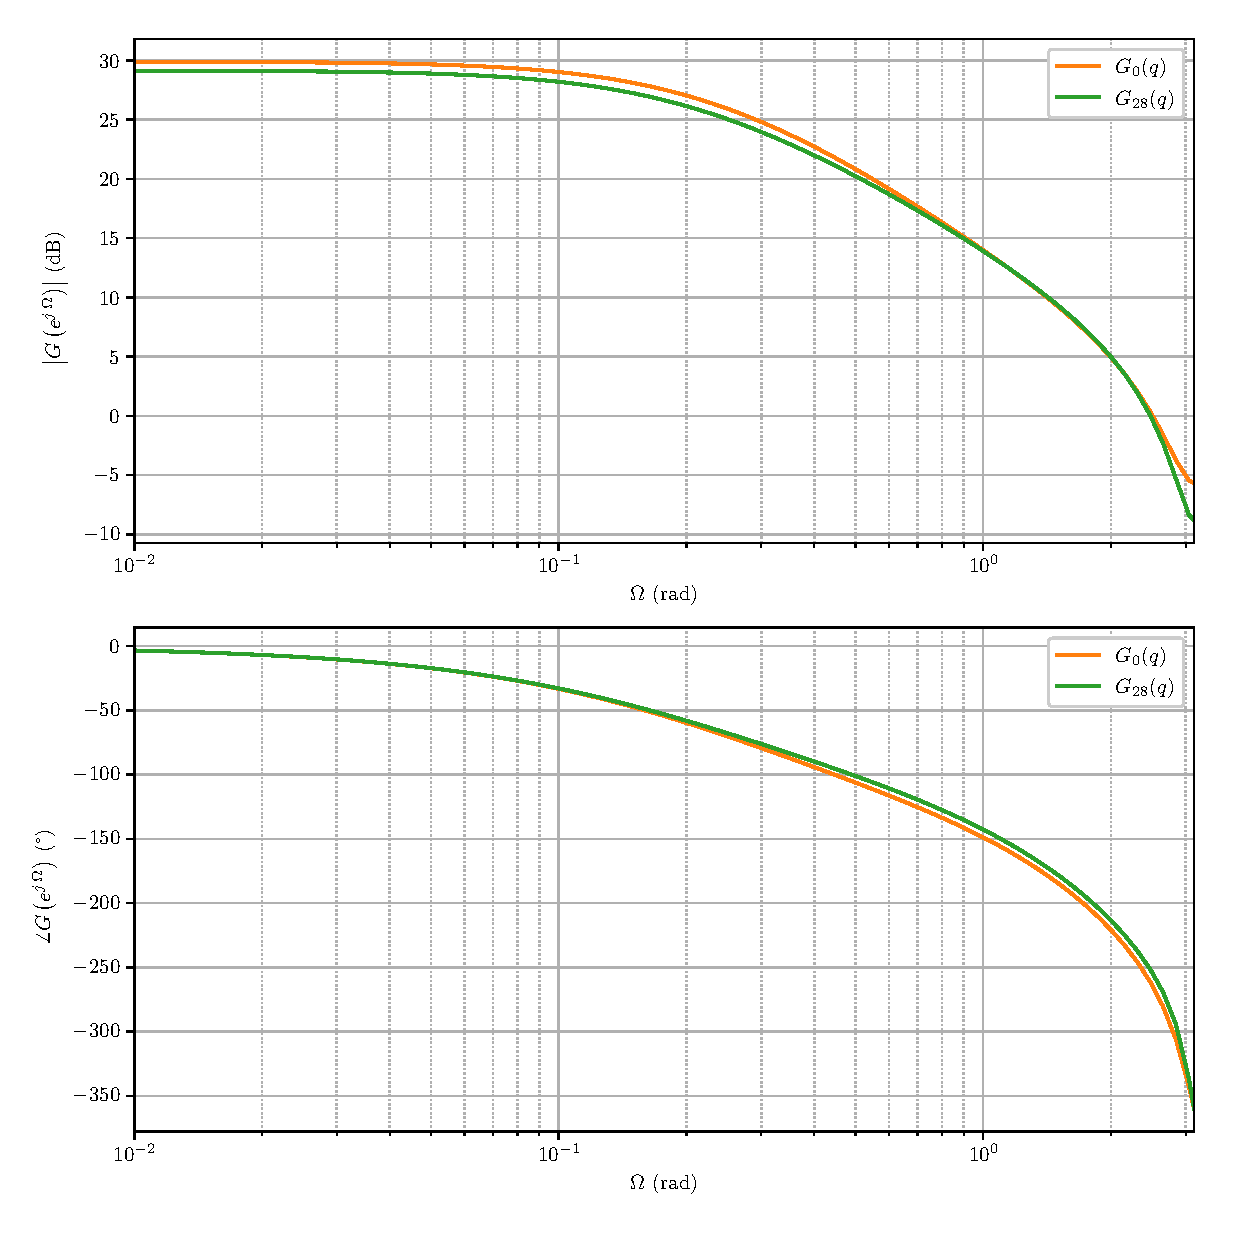
\includegraphics[width=\linewidth]{bode_G_28}
  \caption{Resposta em frequências de $G(q)$ a partir da identificação com o menor modelo de ordem completa.}
  \label{fig:bode-system-complete}
\end{figure}

\begin{figure}[!htbp]
  \centering
  \includegraphics[width=\linewidth]{bode_H_28}
  \caption{Resposta em frequências de $H(q)$ a partir da identificação com o menor modelo de ordem completa.}
  \label{fig:bode-noise-complete}
\end{figure}

\section{Conclusões}

A determinação da classe do modelo é um desafio ao projetista, ainda mais quando a ordem do sistema a ser identificado é desconhecida.
O erro quadrático médio de predição e o critério de informação de Akaike permitem avaliar a qualidade dos modelos obtidos.

Tendo sido realizada uma única identificação por classe, sempre a partir do mesmo conjunto de dados de identificação e validação, os resultados têm um fator considerável de aleatoriedade.
A aleatoriedade poderia ser reduzida com a divisão do conjunto de dados em múltiplos subconjuntos de identificação e validação --- procedimento este denominado validação cruzada --- e posterior comparação dos vários resultados obtidos para cada classe.

\bibliographystyle{IEEEtran}
\bibliography{bib/book, bib/misc, bib/controlIEEE}

\end{document}
